\documentclass[tikz,border=2pt]{standalone}
\usepackage{tikz}
\usetikzlibrary{arrows.meta}
\begin{document}
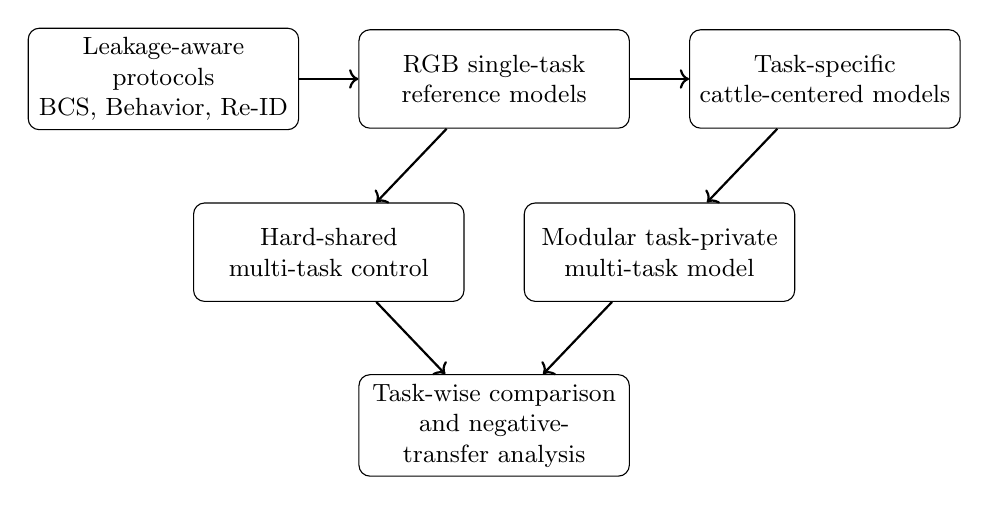
\begin{tikzpicture}[
  box/.style={draw,rounded corners,align=center,text width=3.2cm,minimum height=1.25cm,font=\small},
  arrow/.style={->,thick}
]
\node[box] (protocols) at (0,0) {Leakage-aware protocols\\BCS, Behavior, Re-ID};
\node[box] (rgb) at (4.2,0) {RGB single-task\\reference models};
\node[box] (centered) at (8.4,0) {Task-specific\\cattle-centered models};
\node[box] (e1) at (2.1,-2.2) {Hard-shared\\multi-task control};
\node[box] (e3) at (6.3,-2.2) {Modular task-private\\multi-task model};
\node[box] (synthesis) at (4.2,-4.4) {Task-wise comparison\\and negative-transfer analysis};
\draw[arrow] (protocols) -- (rgb);
\draw[arrow] (rgb) -- (centered);
\draw[arrow] (rgb) -- (e1);
\draw[arrow] (centered) -- (e3);
\draw[arrow] (e1) -- (synthesis);
\draw[arrow] (e3) -- (synthesis);
\end{tikzpicture}
\end{document}